\documentclass[12pt]{article}
\usepackage{lecture}
\usepackage{graphics}
\usepackage{epstopdf}
\usepackage{html}
\usepackage{url}

\newcommand{\qtl}{{\tt QTL Cartographer}}

\newcommand{\copyrightYears}{2001-2010}

\title{Mapping Quantitative Trait Loci with QTL Cartographer}

\begin{document}

\maketitle

\thispagestyle{first}

\section*{Introduction}

There are two stages to making a QTL map for a particular trait
(once you've scored tens or hundreds of marker loci in tens or
hundreds of $F_2$ or backcross progeny):

\begin{enumerate}

\item Construct a genetic map of your markers.

\item Feed the genetic map, marker data, and phenotype data into QTL
Cartographer and run the analysis.

\end{enumerate}

\noindent Although constructing the genetic map of your markers is
really important step, we're not going to talk about it further. It
is, after all, simply an elaboration of classical Mendelian
genetics.\footnote{Although it gets a {\it lot\/} more complicated
  when you're dealing with tens or hundreds of markers, and you don't
  even know which ones belong on which chromosomes!} We're going to
focus on the second step.

\section*{The data}

The input data format for QTL Cartographer is fairly involved, but
it's well documented. If this were a course in QTL analysis, I'd
expect you to become fully conversant with the input formats and their
meanings. Fortunately for you, I don't expect that at all. In fact,
I'm not even going to ask you to run a QTL analysis.\footnote{We're
  going to run an association analysis instead.} Still, it's useful to
take a brief look at the data format, so you can see the type of data
that's involved in a QTL analysis. You can download the data file I'm
using ({\tt realdat\_In.mcd}) from
\htmladdnormallink{http://darwin.eeb.uconn.edu/eeb348/supplements-2006/Maize.mcd}{http://darwin.eeb.uconn.edu/eeb348/supplements-2008/Maize.mcd}
and open it in {\tt WinQTLCart}. When you do, you'll find the
following description of the data on your screen:

{\small
\begin{verbatim}
#FileID 901540162
#bychromosome
/* One way to make comment
   on data source file */
-type position //default is interval
-function 1 //default is 1
-Units cM //default is cM
-chromosomes 1
-maximum 12 
-named yes
-start
-Chromosome C1
// Another way to comment
  Mk01_01         0.0000
  Mk01_02        37.8000
  Mk01_03        49.1000
  Mk01_04        59.8000
  Mk01_05        62.8000
  Mk01_06        86.7000
  Mk01_07        92.7000
  Mk01_08       108.2000
  Mk01_09       112.5000
  Mk01_10       134.6000
  Mk01_11       140.0000
  Mk01_12       149.8000
-stop

\end{verbatim}
}

There is one chromosome represented in our marker data (labeled {\tt
c1}). The last table gives the name of each marker, in linkage map
order, and the distance to the next marker.

The crossing data follows in the next section and is quite a bit more
complicated.

{\scriptsize
\begin{verbatim}
---------------------------------------------------
#bycross
-SampleSize 171 //Individual number
-Cross SF2 //default is B1
-traits 1
-missingtrait . //default is . and may use -losttrait
-case yes
-TranslationTable //can omit
  AA    2     2  //default 2
  Aa    1     1  //default 1
  aa    0     0  //default 0
  A-    12    12 //default 12
  a-    10    10 //default 10
  --    -1    -1 //default -1
-start markers
Mk01_01 2  1  1  1  0  1  2  0  1  0  1  2  2  1  1  1  1  2  0  2 
 0  2  1  1  2  1  0  0  2  2  1  2  1  1  1  0  1  1  1  0 
 1  2  2  1  2  0  0  0  1  2  1  2  1  1  0  1  0  1  1  0 
 1  2  2  0  1  1  1  0  1  0  2  1  1  1  2  1  2  2  0  2 
 0  0  1  1  2  0  1  1  1  1  1  2  1  1  1  2  1  0  1  0 
 0  2  2  0  1  0  1  2  0  2  1  2  2  2  1  1  2  0  1  0 
 0  1  1  2  2  0  1  1  1  1  1  2  0  0  0  2  1  0  0  1 
 1  1  0  2  1  1  1  0  1  1  1  0  1  1  2  1  0  1  1  1 
 1  2  1  1  1  1  2  1  0  1  2 
    
    .
    .
    .

Mk01_12 0  1  2  2  1  0  2  2  1  0  0  1  1  1  2  1  0  0  1  0 
 0  0  2  0  1  0  2  1  1  1  2  1  0  1  2  0  2  2  0  1 
 1  2  1  2  1  1  1  1  1  2  1  0  2  2  1  1  0  1  1  2 
 2  1  1  1  2  1  0  2  1  1  1  0  2  1  1  0  2  2  2  2 
 0  1  2  1  1  1  0  1  2  0  1  1  1  2  0  2  0  1  1  2 
 1  0  2  1  0  1  1  1  1  1  1  1  1  1  0  1  1  2  0  2 
 2  1  0  1  1  1  1  1  2  0  1  2  1  1  1  0  0  0  1  2 
 1  2  1  0  2  2  2  1  1  0  1  1  2  1  2  0  0  1  1  1 
 0  0  2  1  1  2  1  2  1  1  0 
-stop markers
-start traits
Trait_1  6.2500 3.0000 3.0000 4.0000 3.0000 3.7500 8.2500 2.5000 4.2500 4.5000 6.0000 3.2500 5.5000 7.2500 5.5000 
4.0000 2.7500 7.5000 6.0000 4.7500 2.7500 5.5000 1.7500 5.0000 4.0000 4.0000 2.0000 3.0000 4.7500 3.7500 
5.7500 8.0000 3.0000 2.2500 3.5000 6.7500 2.2500 3.5000 6.2500 1.5000 3.5000 4.0000 6.2500 3.0000 7.2500 
1.7500 7.2500 1.2500 7.2500 6.7500 6.5000 2.7500 3.5000 4.2500 3.0000 6.2500 1.5000 3.2500 4.7500 2.2500 
2.7500 5.0000 3.0000 5.0000 3.2500 6.7500 6.2500 1.2500 2.7500 3.0000 8.2500 3.5000 2.7500 7.2500 5.7500 
5.2500 6.7500 6.0000 1.5000 3.5000 5.0000 5.0000 3.7500 4.0000 4.5000 1.5000 7.5000 3.2500 7.5000 2.7500 
5.5000 2.5000 3.0000 5.0000 3.0000 2.7500 2.7500 3.5000 7.0000 1.7500 2.7500 3.5000 6.7500 2.7500 3.0000 
2.7500 2.7500 5.7500 2.7500 6.5000 1.7500 4.7500 4.7500 3.5000 5.5000 6.5000 5.0000 4.7500 2.2500 2.0000 
4.2500 4.2500 6.0000 5.2500 6.0000 3.5000 2.2500 3.0000 4.5000 4.0000 8.2500 4.7500 1.5000 1.2500 2.2500 
6.7500 7.5000 2.5000 2.0000 2.5000 2.5000 7.5000 2.0000 4.0000 2.7500 3.0000 3.7500 6.5000 4.2500 3.5000 
1.7500 4.0000 5.2500 2.5000 7.2500 2.7500 1.0000 7.5000 4.5000 5.7500 4.5000 4.5000 3.5000 5.5000 1.7500 
5.7500 4.0000 3.5000 5.5000 3.0000 5.7500 
-stop traits
-quit
-end
\end{verbatim}
}

After some basic information about the structure of the data the line
{\tt -start markers} denotes the beginning of the marker
information. The genotype of the 171 individuals scored is entered
following the label form the marker. When the marker data is finished
({\tt -stop markers}), we start the trait information ({\tt -start
traits}). After a short label describing the trait, the information
for each individual is entered.

\section*{Running an analysis}

\qtl{} was originally written for use on Unix workstations. The main
documentation refers to a series of programs that can be used for a
QTL analysis. If you get serious about QTL analyses, you'll need to
understand each of those programs thoroughly. The design of \qtl{}
reflects the Unix philosophy. Instead of writing one, big, monolithic
program that does everything, the authors of \qtl{} wrote a series of
small tools that work well together, and allow users to work with them
individually as they see fit. That's great for complex analyses, but
it makes learning the package a little difficult. For our purposes,
we'll stick with the simpler interface provided by {\tt
  WinQTLCart}. After loading the data with {\tt File->Open} and
hitting the {\tt Verify} button, your screen should look something
like Figure~\ref{fig:qtl-data-loaded}.

\begin{figure}
\begin{center}
\resizebox{!}{8cm}{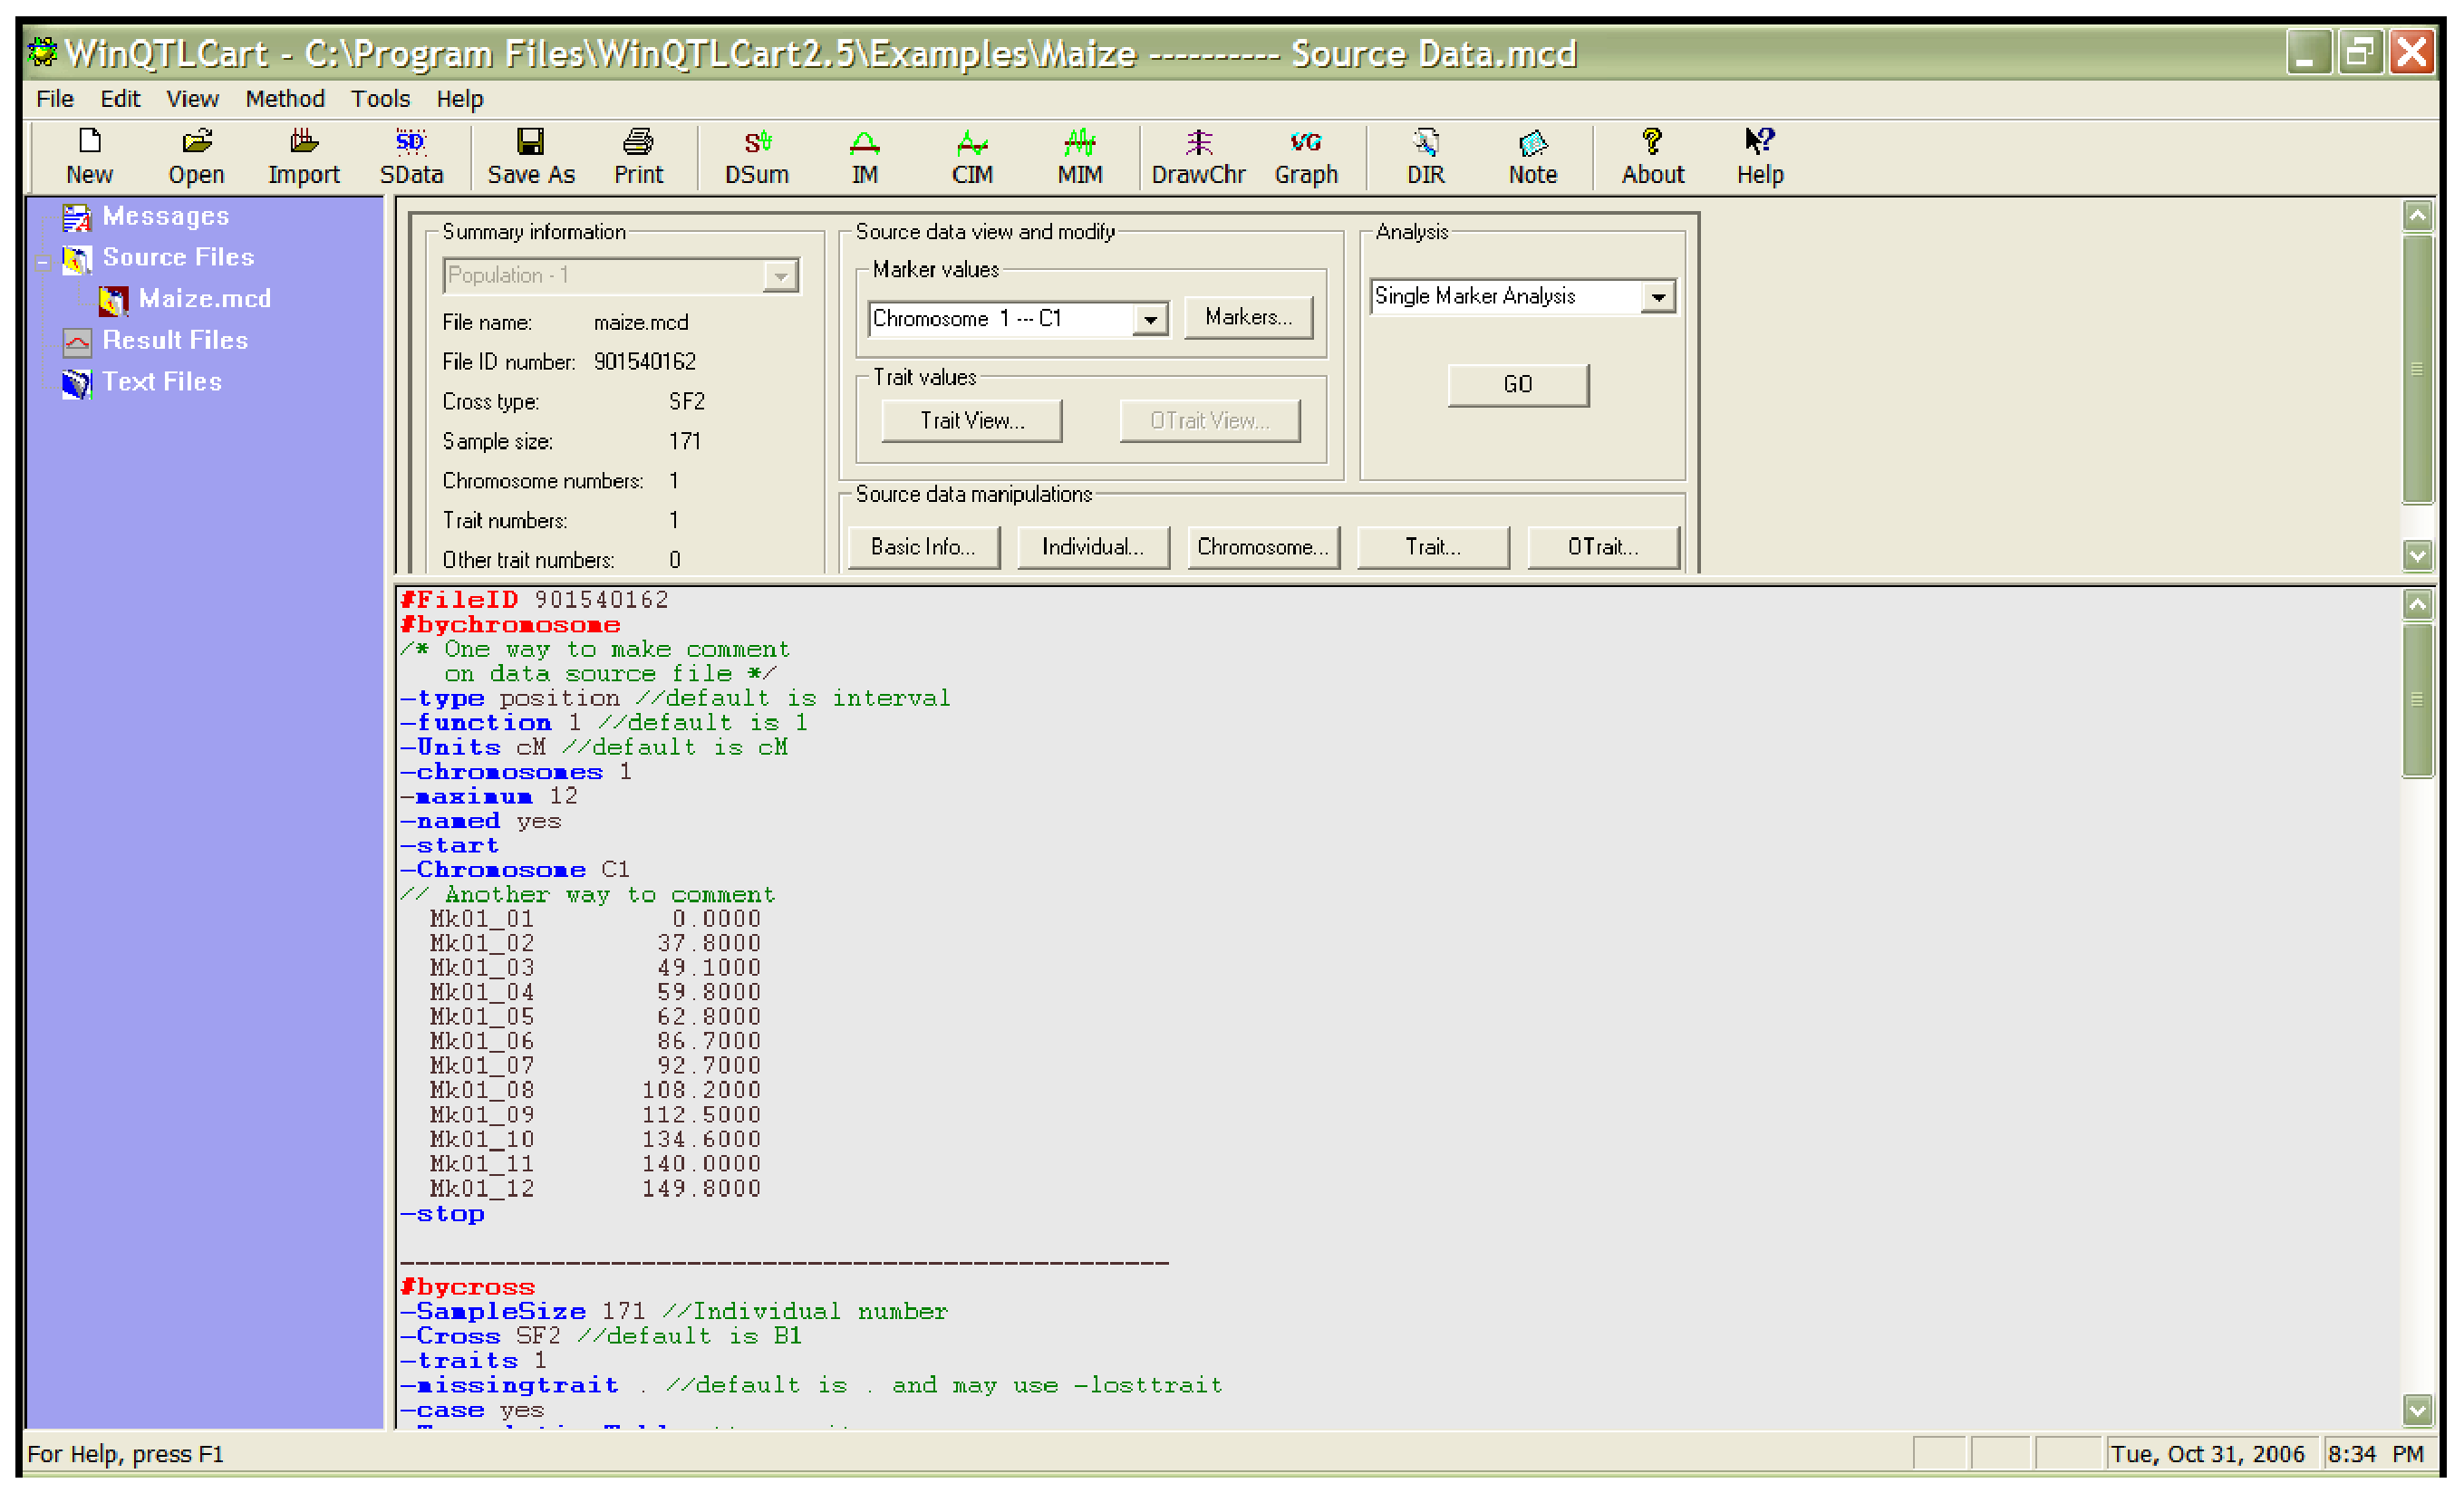
\includegraphics{qtl-data-loaded.eps}}
\end{center}
\caption{Screenshot of {\tt WinQTLCart} after the data in {\tt
    Maize.mcd} has been loaded.}\label{fig:qtl-data-loaded}
\end{figure}

You could modify information about the traits, the genetic map, or the
crosses using the buttons if you chose to, but we'll assume that
everything is as it should be so that you don't have to worry about
that. If you now hit the {\tt DrawChr} button, you'll get a nice
graphic showing you a linkage map of the genetic markers you're
using~(Figure~\ref{fig:qtl-marker-map}).

\begin{figure}
\begin{center}
\resizebox{!}{6cm}{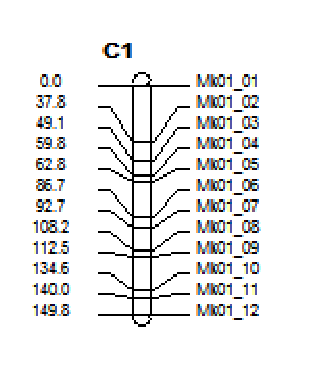
\includegraphics{qtl-marker-map.eps}}
\end{center}
\caption{Map of genetic markers for the sample data set used in this analysis.}\label{fig:qtl-marker-map}
\end{figure}

Once you've made it this far, running the analysis is as simple as
pulling down the {\tt Method} menu and selecting the method you want
to use. We don't have time to discuss the differences among the
methods in detail, but I'll briefly summarize the methods here:

\begin{description}

\item[Single Marker Analysis] Select {\tt Single Marker Analysis} and
  press ``Go''  (or select {\tt Method->Single Marker Analysis} from the menu).

\begin{itemize}

\item If you push the {\tt View info...} button in the {\tt Single
    Marker Analysis} box, you'll get a linear regression analysis of
  the relationship between phenotype and marker genotype for each
  marker individually. This analysis tells us that there's a
  significant positive relationship between genotype and phenotype for
  the first three markers.\footnote{Remember that $AA$ is 2, $Aa$ is
    1, and $aa$ is 0, so a positive relationship means that $A$ is
    associated with increased values of the trait.}

\item If you push the {\tt View info...} button in the {\tt
  Statistical Summary} box, you'll get summary statistics on the
  pattern of trait variation in the mapping population and on the
  pattern of segregation at the marker loci, i.e., whether they follow
  Mendelian expectations. The values should follow a $\chi^2$
  distribution with 1 degree of freedom. In this case, the genotype
  proportions in our mapping population all appear to be consistent
  with Mendelian expectations.

\end{itemize}

\item[Interval mapping] When you select this menu item the analysis
  performed is simple interval mapping of the type I've already
  described. One slight complication is that because you're doing a
  lot of statistical tests when doing a QTL analysis, you have to take
  account of that fact in choosing a threshold value of the likelihood
  ratio statistic for declaring that you've found a QTL. You can
  accept the default value, put in one of your own choosing, or select
  one through permutations (which will take the longest, but should
  produce the most reliable choice). After you push the {\tt OK}
  button, you'll see the program counting down from the number of
  permutations you asked for to zero. 

  The other parameter you may want to change is the {\tt Walk
  speed}. That's the parameter that determines the interval along the
  map at which QTL calculations are done. If you have a very dense
  map, you can set the interval to be quite small, and you'll have a
  much more precise idea of where any QTLs you locate may be, but it
  will take the program much longer to do the calculations. We'll
  leave the walk speed at the default {\tt 2cm} for this example.

  Once the permutations have finished, {\tt WinQTLCart} will
  automatically enter the new threshold value, and you're ready to
  look for a QTL. Hit the {\tt Start} button, and you'll soon see
  something like Figure~\ref{fig:qtl-interval-results}

\begin{figure}
\begin{center}
\resizebox{!}{6cm}{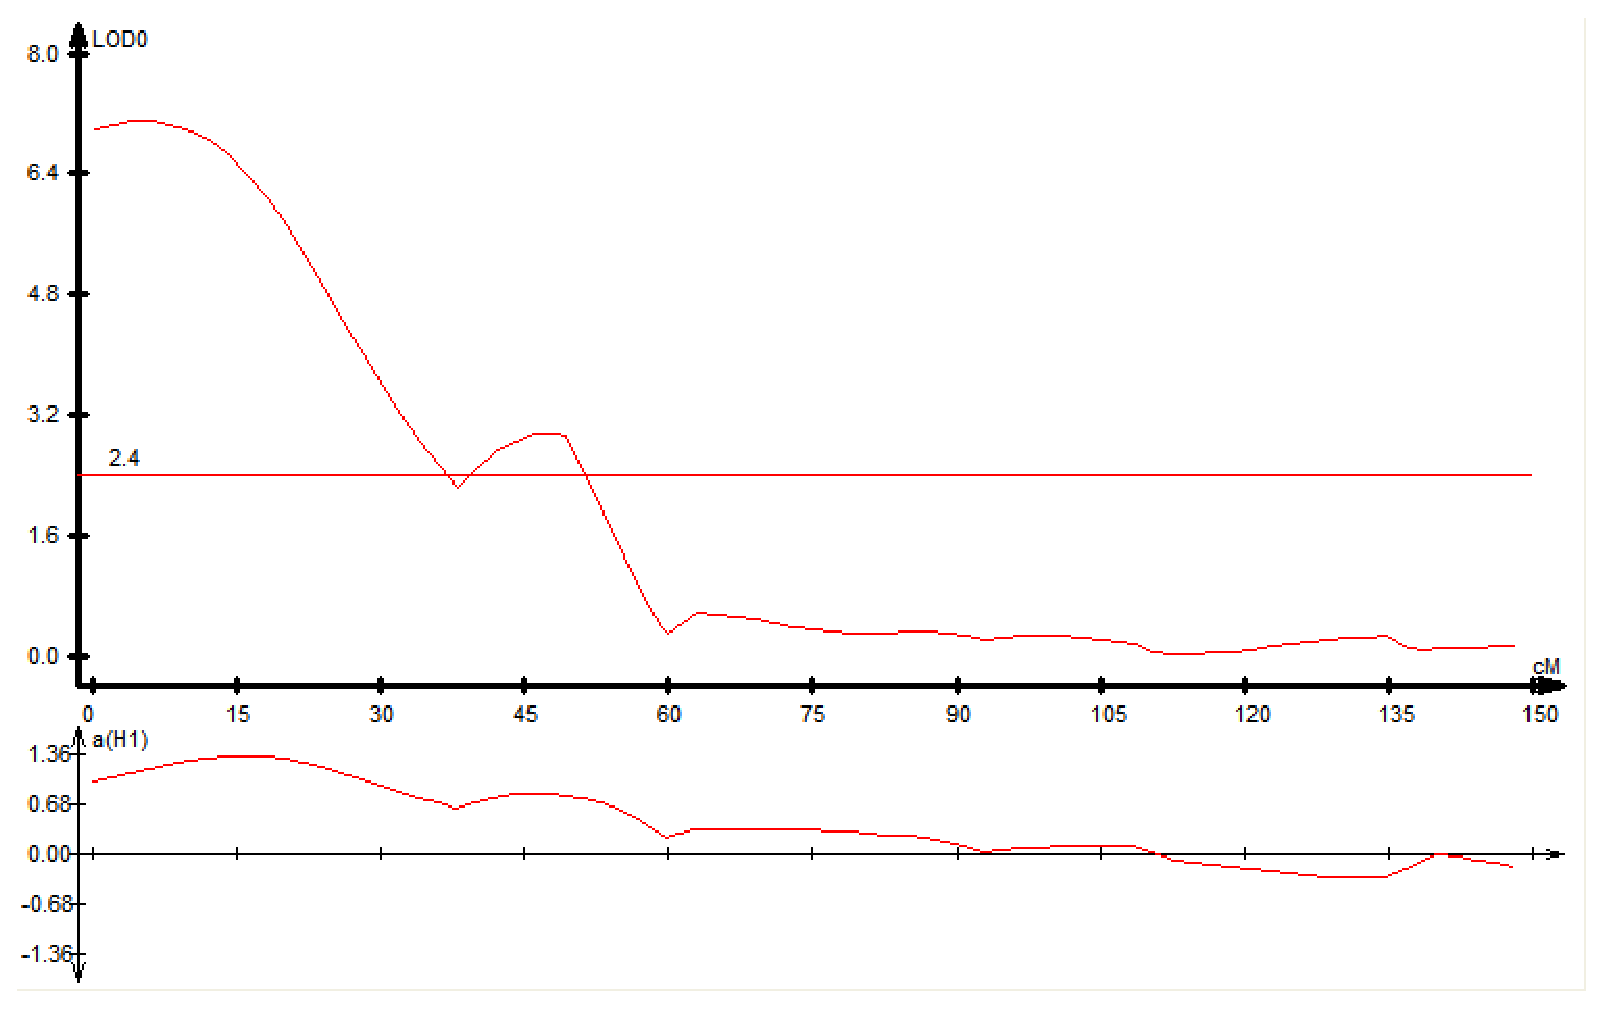
\includegraphics{qtl-interval-results.eps}}
\end{center}
\caption{Interval mapping results for the sample data. I turned off
    the background using {\tt Settings->Show Colorful Background}
    option to make the background ywhite.}\label{fig:qtl-interval-results}
\end{figure}

This figure suggests that a QTL is present at about 6cm from the
left end of the chromosome. Finding the corresponding line in the
output (position 0.0601) we see that the additive effect of the $A$
allele at this locus is estimated to be 1.16, the dominance
deviation (the extent to which the heterozygote departs from
intermediacy) is 0.0388, and that this QTL accounts for about 22\% of
the variance in the trait.\footnote{I'm getting this from the columns
  for H3:a, H3:d, and R2(0:3), respectively, for reasons I'll explain
  in class.}

\item[Composite interval mapping] The options available under
  composite interval mapping are very similar to those for interval
  mapping. That's because the underlying statistical model is very
  similar. In fact the only difference is the {\tt CIM} is attempting
  to statistically control for the genotype at markers other than
  those immediately flanking the candidate QTL. The results are in
  Figure~\ref{fig:qtl-composite-results}. They look pretty similar,
  but notice that the peak is at 0cm and the one at about 47cm barely
  reaches the threshold.

\begin{figure}
\begin{center}
\resizebox{!}{6cm}{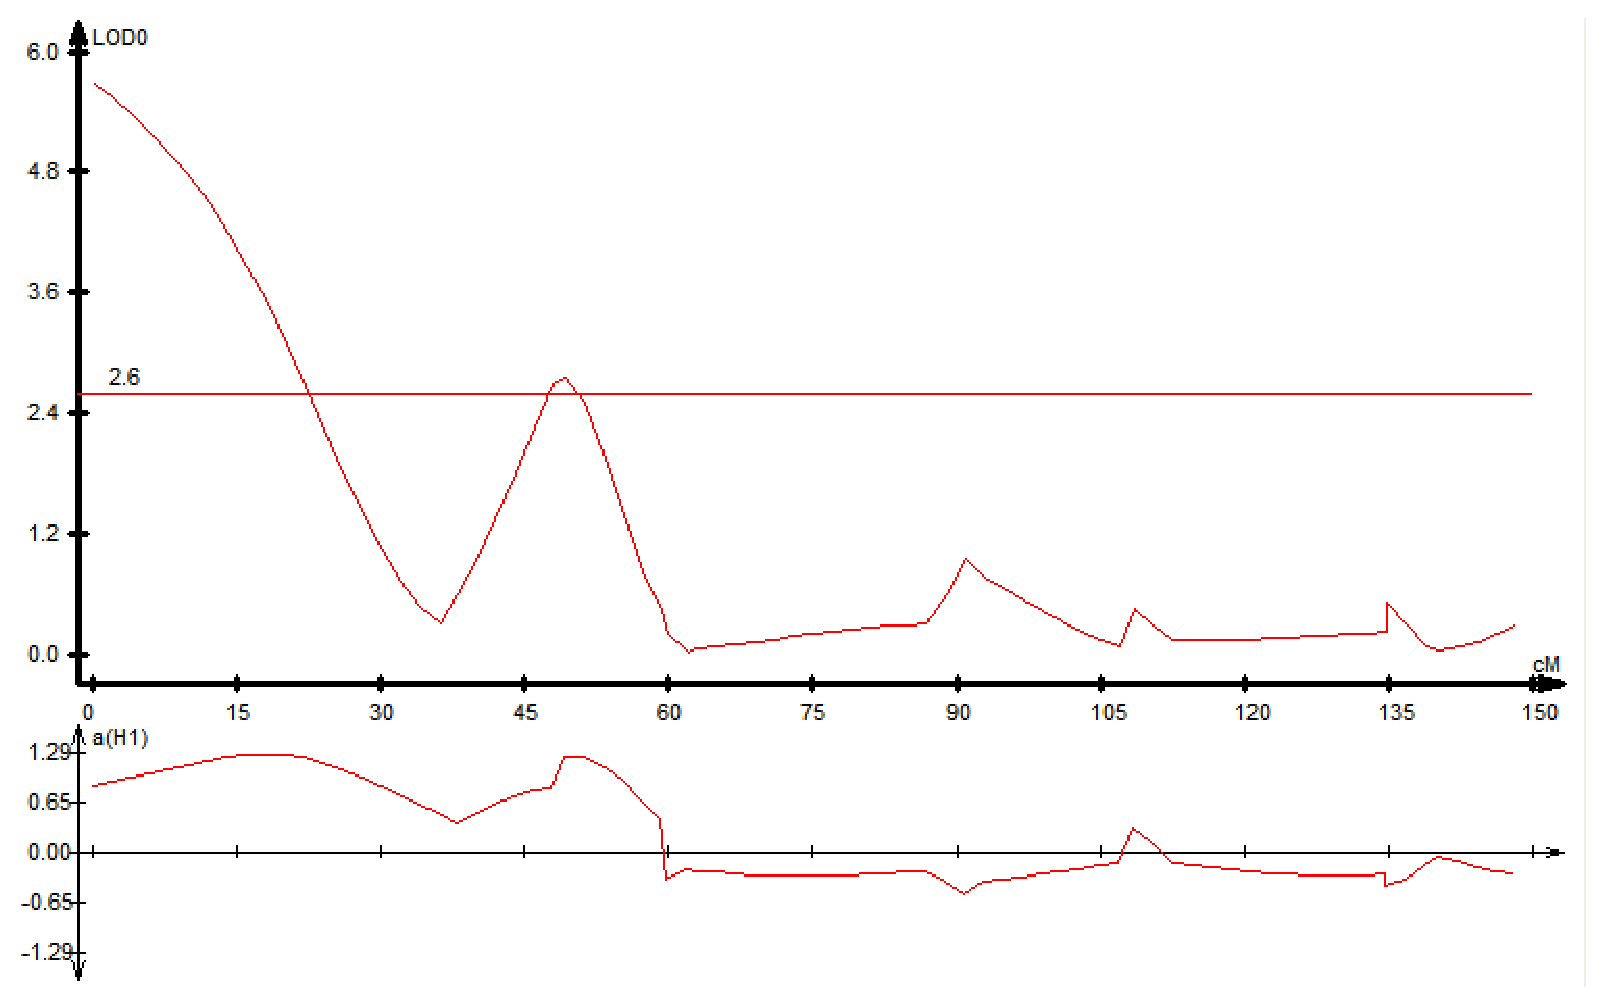
\includegraphics{qtl-composite-results.eps}}
\end{center}
\caption{Results of a composite interval mapping analysis of the
  sample data.}\label{fig:qtl-composite-results}
\end{figure}

\item[Multiple interval mapping] Multiple interval mapping is a still
  more sophisticated method of mapping. It allows you to identify more
  than one QTL and to refine your analyses as you go along. One nice
  feature is that it puts a nice summary of the results up in the
  window. The data we've been using give us a QTL at 3cm, with an
  additive effect of 1.15, and a dominance deviation of
  0.069. Running the summary statistic report, we find (again) that
  this QTL explains about 19\% of the phenotypic variance.

\item[Bayesian interval mapping]\footnote{I'll bet you knew there was
  a Bayesian version coming, didn't you?} Although Bayesian interval
  mapping appears on the menu, and an analysis will run, I haven't had
  time to figure out how to interpret the results yet, so we won't
  talk about it.

\end{description}

\section*{Interpreting the output files}

When analyzing an $F_2$ design using composite interval mapping,
\qtl{} reports 21 columns of information for each position in the walk
along the chromosomes. Before enumerating those statistics, it's
useful to point out that there are four hypotheses being examined at
each position:

\begin{itemize}

\item $H_0$: $a=0, d=0$ -- Both the additive allelic effect and the
  dominance deviation are zero.

\item $H_1$: $a \ne 0, d=0$ -- The additive allelic effect is
  distinguishable from zero, but the dominance deviation is zero.

\item $H_2$: $a=0, d \ne 0$ -- The additive allelic effect is zero,
  but the dominance deviation is distinguishable from zero. 

\item $H_3$: $a \ne 0, d \ne 0$ -- Both the additive allelic effect
  and the dominance deviation are zero.

\end{itemize}

\noindent Many of the 21 columns in the output correspond to
comparisons among these hypotheses or to estimates of additive and
dominance effects under a particular hypothesis. Here's what each
column in the output corresponds to:

\begin{enumerate}

\item Chromosome on which the test position is located.

\item Left flanking marker associated with the test position.

\item Absolute position of the test position from the left telomere of
  this chromosome (in Morgans).

\item Likelihood-ratio test statistic for $H_3$ {\it versus\/} $H_0$. 

\item Likelihood-ratio test statistic for $H_3$ {\it versus\/} $H_1$. 

\item Likelihood-ratio test statistic for $H_3$ {\it versus\/} $H_2$. 

\item Estimate of the additive allelic effect, $a$, under $H_1$.

\item Estimate of the additive allelic effect, $a$, under $H_3$.

\item Estimate of the dominance effect, $d$, under $H_2$.

\item Estimate of the dominance effect, $d$, under $H_3$.

\item Likelihood-ratio test statistic for $H_1$ {\it versus\/} $H_0$. 

\item Likelihood-ratio test statistic for $H_2$ {\it versus\/} $H_0$. 

\item $r^2$ for $H_1$ {\it versus\/} $H_0$ -- The extent to which
  $H_1$ reduces the residual variance,\footnote{Remember that for
    composite interval mapping, we fit a regression of phenotype on
    backgrnound genotype before running the analysis. The residual
    variance is the variance {\it not\/} explained by this
    regression.} relative to the total variance.\footnote{The total
    variance is just what it says, the total observed phenotypic
    variance. $1-r^2$ is the proportion of phenotypic variance
    accounted for by the QTL at this position.}

\item $r^2$ for $H_2$ {\it versus\/} $H_0$ -- The extent to which
  $H_2$ reduces the residual variance, relative to the total
  variance. 

\item $r^2$ for $H_3$ {\it versus\/} $H_0$ -- The extent to which
  $H_3$ reduces the residual variance, relative to the total
  variance. 

\item $r^2_t$ for $H_1$ {\it versus\/} $H_0$ -- The extent to which
  $H_1$ reduces the total variance.\footnote{$1-r^2_t$ is the
    proportion of phenotypic variance accounted for by the QTL at this
    position and the background genotype.} 

\item $r^2_t$ for $H_2$ {\it versus\/} $H_0$ -- The extent to which
  $H_2$ reduces the total variance.

\item $r^2_t$ for $H_3$ {\it versus\/} $H_0$ -- The extent to which
  $H_3$ reduces the total variance.

\item A test statistic, $S$, for normality of the residuals under
  $H_1$.\footnote{$S$ is distributed as a $\chi^2$ with two degrees of
    freedom.}

\item A test statistic, $S$, for normality of the residuals under $H_2$.

\item A test statistic, $S$, for normality of the residuals under $H_3$.

\end{enumerate}

\ccLicense

\end{document}


